16.	如图所示,在长方形ABCD中,有一个最大的圆O,已知AB=3厘米,BC=4厘米,两只蚂蚁同时从点M出发,第一只蚂蚁沿圆周以每秒3毫米的速度爬行,第二只蚂蚁沿长方形的边以每秒5毫米的速度爬行,请问:哪只蚂蚁先回到出发点M?早几秒钟?

\begin{flushright}

    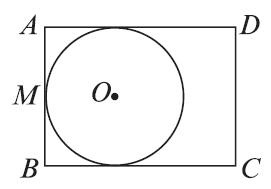
\includegraphics[height=3.25cm]{lib/image/MJA04020116.png}

\end{flushright}



